\chapter{Greedy Algorithm}

\section{Maximal Matching}

\begin{algoprob}
	\problemtitle{Maximal Matching}
	\probleminput{Graph $G=(V,E)$}
	\problemquestion{Find a maximal matching $M\subseteq E$ of $G$}
\end{algoprob}
Before diving into the algorithm to find a matching or maximal matching we first define what is a matching.
\begin{Definition}{Matching}{}
	For a graph $G=(V,E)$ a matching $M\subseteq E$ is a set of edges such that no two edges in $M$ are incident on same vertex.
\end{Definition}
\begin{Definition}{Maximal Matching}{}
	For a graph $G=(V,E)$ a matching $M\subseteq E$ is maximal if it cannot be extended and still by adding an edge.
\end{Definition}
There is also a maximum matching which can be easily understood from the name:
\begin{Definition}{Maximum Matching}{}
	For a graph $G=(V,E)$ a matching $M\subseteq E$ is maximum if it is maximal and has the maximum size among all the maximal matchings.
\end{Definition}

\begin{idea*}
	The idea is to create a maximal matching we will just go over each edge one by one and check if after adding them to the set $M$  the matching property still holds. 
\end{idea*}
\begin{algorithm}
	\SetKwComment{Comment}{// }{}
	\DontPrintSemicolon
	\KwIn{Graph $G=(V,E)$}
	\KwOut{Maximal Matching $M\subseteq E$ of $G$}
	\Begin{
	$M\longleftarrow \emptyset$\;
	Order the edges $E=\{e_1,\dots, e_k\}$ arbitrarily\;
	\For{$e\in E$}{\If{$M\cup \{u\}$ is matching}{$M\longleftarrow M\cup \{e\}$}}
	\Return{$M$}	
}
\caption{\prb{Maximal-Matching}}
\end{algorithm}

\begin{question}{}{}
		Do we always get the largest possible matching?
\end{question}
\solve{ Clearly algorithm output is not optimal always. We get a maximal matching sure. But we don't get a maximum matching always. For example the following graph
	\begin{center}
		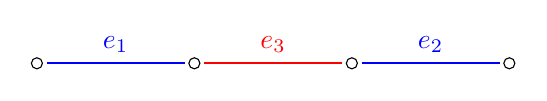
\begin{tikzpicture}
			\draw (-2,0) circle (2pt) node (A){};
			\draw (0,0) circle (2pt) node (B){};
			\draw (2,0) circle (2pt) node (C){};
			\draw (4,0) circle (2pt) node (D){};
			\draw[blue, thick] (A) -- node[midway, above]{$e_1$} (B);
			\draw[red, thick] (B) -- node[midway, above]{$e_3$}(C);
			\draw[blue, thick] (C) -- node[midway, above]{$e_2$} (D);
		\end{tikzpicture}
	\end{center}
	If we start from $e_1$ we get the matching $\{e_1.e_2\}$ which is maximum matching but if we start from $e_3$ then we get only the maximal matching $\{e_3\}$ which is not maximum.}

 Since the algorithm output may not be optimal always we can ask the following question
 \begin{question}{}{}
 	How large is the matching obtained compared to the maximum matching?
 \end{question}
This brings us to the following result:

\begin{Theorem}{}{}
	For any graph $G$ let the greedy algorithm obtains the matching $M$ and the maximum matching is $M^{\star}$. Then $$|M|\geq \frac12|M^\star|$$
\end{Theorem}
\begin{proof}
	Consider an edge $e\in M^{\star}$ but $e\notin M$. Since $e$ wasn't  picked in $M$, $\exs\ e'\in M\setminus M^{\star}$ such that $e$ and $e'$ are incident on same vertex. Thus define the function $f:M^{\star}\to M$ where $$f(e)=\begin{cases}
		e&\text{when $e\in M$}\\
		e' & \text{when $e\in M^{\star}\setminus M$ where $e'\in M\setminus M^{\star}$ such that $e'\cap e\neq \emptyset$}
	\end{cases}$$

Now note that there are at most  two edges in $M^{\star}$ that are adjacent to an edge $e'\in M$ which will be mapped to $e'$. Hence $$|M\setminus M^{\star}|\geq \frac12 |M^{\star}\setminus M|$$Therefore $|f^{-1}(e')|\leq 2$ $\forall\ e'\in M$. Hence $$|M^\star|=|M\cap M^{\star}|+|M^{\star}\setminus M|\leq |M\cap M^{\star}|+2|M\setminus M^{\star}|\leq 2|M|$$Therefore we have the result $|M|\geq \frac12|M^{\star}|$. 
\end{proof}
\begin{alternate-proof} 
	Let $M_1$ and $M_2$ are two matchings. Consider the symmetric difference $M_1\triangle M_2$.  This consists of edges that are in exactly one of $M_1$ and $M_2$. Now in $M\triangle M^{\star}$ we have the following properties:
	\begin{enumerate}[label=(\alph*)]
		\item Every vertex in $M\triangle M^{\star}$ has degree $\leq 2\implies $ Each component is a path or an even cycle. 
		\item The edges of $M$ and $M^{\star}$ alternate. 
			\end{enumerate}
		Now we will prove the following property about the connected components of $M\triangle M^{\star}$.
		
\begin{center}
					
	\begin{minipage}{0.9\textwidth}
			\textit{\textbf{Claim:}}\hspace{1em} No connected component is a single edge. 
		
		\begin{proof}
			This is because let $e$ be a connected component. So the two edges $e_1,e_2$ which are adjacent to $e$,  they are either in both $M$ and $M^{\star}$ or not in $M$ and $M^{\star}$. The former case is not possible because then $e_1,e_2,e$ are all in either $M$ or $M^{\star}$ which is not possible as they do not satisfy the condition of matching. For the later case since $M^{\star}$ is maximal matching, $e\in M^{\star}$. Then $e\notin M$. That means $e,e_1,e_2\notin M$ which is not possible since $M$ is also a maximal matching. Therefore no connected component is a single edge.
		\end{proof}
	\end{minipage}
\end{center}

	
		Therefore every path has length $\geq 2$. Therefore ratio of $\#$ edges of $M$ to $\#$ edges of $M^{\star}$ in a path is $\leq 2$. And for cycles we have $\#$ edges of $M=\#$ edges of $M^{\star}$. So in every connected component $C$ of $M\triangle M^{\star}$ the ratio $\frac{|M^{\star}\cap C|}{|M\cap C|}\leq 2$. Therefore we have $$\frac{|M^{\star}|}{|M|}=\frac{|M\cap M^{\star}|+\sum\limits_{C}|M^{\star}\cap C|}{|M\cap M^{\star}|+\sum\limits_{C}|M\cap C|}\leq 2$$Hence we have $|M|\geq \frac12|M^\star|$.
		

\end{alternate-proof}
\section{Huffman Encoding}
\begin{algoprob}
	\problemtitle{Huffman Coding}
	\probleminput{$n$ symbols $A=(a-1,\dots, a_n)$ and their frequencies $P=(f_1,\dots, f_n)$ of using symbols}
	\problemquestion{Create a binary encoding such that: \begin{itemize}[itemsep=-0.2cm]
			\item Prefix Free: The code for one word can not be prefix for another code
			\item Minimality: Minimize $\prb{Cost}(b)=\sum\limits_{i=1}^n f_i\cdot \prb{Len}(b(a_i))$ where $b:A\to \{0,1\}^*$ is the binary encoding
	\end{itemize}}
\end{algoprob}

Assignment of binary strings can also be scene as placing the symbols in a binary tree where at any node $0$ means left child and $1$ means right child. Then the first condition implies that there can not be two codes which lies in the same path from the root to a leaf. I.e. it means that all the codes have to be in the leaves. Then the length of the binary coding for a symbol  is the height of the symbol in the binary tree. 

We can think the frequencies as the probability of appearing for a letter. We denote the probability of appearing of the letter $a_i$ by $p(a_i)\coloneqq \frac{f_i}{\sum\limits_{i=1}^nf_i}$. So the we can see the updated cost function $$\prb{Cost}(b)=\sum\limits_{i=1}^n p(a_i)\cdot\prb{Len}(b(a_i))$$And from now on we will see the frequencies as probabilities and cost function like this

\subsection{Optimal Binary Encoding Tree Properties}
Then our goal is to finding a binary tree with minimum cost where all the symbols are at the leaves. We have the following which establish the optimality of Huffman encoding over all prefix encodings where each symbol is assigned a unique string of bits.
\begin{lemma}{}{least-frequent-max-height}
	In the optimal encoding tree  least frequent element has maximum height.
\end{lemma}
\begin{proof}
	Suppose that is not the case. Let $T$ be the optimal encoding tree and let the least frequent element $x$ is at height $h_1$ and the element with the maximum height is $y$ with height $h_2$ and we have $h_1<h_2$.  Then we construct a new encoding tree $T'$ where we swap the positions of $x$ and $y$. So in $T'$ height of $y$ is $h_1$ and height of $x$ is $h_2$. Then $$\prb{Cost}(T)-\prb{Cost}(T')=(p(x)h_1+p(y)h_2)-(p(x)h_2+p(y)h_1)=(p(x)-p(y))(h_1-h_2)$$Since $p(x)<p(y)$ and $h_1<h_2$ we have $\prb{Cost}(T)-\prb{Cost}(T')>0$. But that is not possible since $T$ is the optimal encoding tree. So $T$ should have the minimum cost. Hence contradiction. $x$ has the maximum height.
\end{proof}

\begin{lemma}{}{complete-tree}
	The optimal encoding binary tree must be complete binary tree. (i.e. every non-leaf node has exactly $2$ children)
\end{lemma}
\begin{proof}
	Suppose $T$ be the optimal binary tree and there is a non-leaf node $r$ which has only one child at height $h$. 
	By \lmref{least-frequent-max-height} the least frequent element $x$ has the maximum height, $h_m$. 
	
	 Then consider the new tree $\hat{T}$ where we place the least frequent element at height $h$ and make it the second child of the node $r$. Then $$\prb{Cost}(T)-\prb{Cost}(\hat{T})=p(x)h_m-p(x)h=p(x)(h_m-h)>0$$But this is not possible as $T$ is the optimal binary tree and it has the minimal cost. Hence contradiction. Therefore the optimal encoding binary tree must be a complete binary tree. 
\end{proof}
\begin{lemma}{}{least-frequents-siblings}
There is an optimal binary encoding tree such that the least frequent element and the second least frequent element are siblings at the maximum height.
\end{lemma}
\begin{proof}
Let $T$ be optimal binary encoding tree. Suppose $x$, $y$ are the least frequent element and the second least frequent element. And suppose $b$, $c$  be two siblings at the maximum height of the tree (There may be many such siblings, and if so pick any such pair.). If $\{x,y\}=\{b,c\}$ we are done. So suppose not. Let the frequencies of $x,y,b,c$ are respectively $p(x),p(y),p(b),p(c)$ and heights of $x,y,b$ are $h_x,h_y$ and $h$ respectively.  WLOG assume $p(x)\leq p(y)$ and $p(b)\leq p(c)$. 

Now since we know $x,y$ have the smallest frequencies we have $p(x)\leq p(b)$ and $p(y)\leq p(c)$. And since $b,c$ have the maximum height we have $h_x,hy\geq h$. So we switch the position of $x$ with $b$ to form the new tree $T'$. And from $T'$ we swap the positions fo $y$ and $c$ to form a new tree $T''$.

\begin{center}
	\begin{tikzpicture}[
		every node/.style={font=\sffamily, align=center, line width=0.15mm},
		level 1/.style={level distance=1cm, sibling distance=2cm},  % Adjusted distance for level 1
		level 2/.style={sibling distance=2cm},   % Adjusted distance for level 2
		square/.style={draw, shape=rectangle, minimum width=0.5cm, minimum height=0.5cm, inner sep=0pt, text width=0.5cm, text centered},
		circle/.style={draw, shape=circle, minimum width=0.5cm, minimum height=0.5cm, inner sep=0pt, text width=0.5cm, text centered},
		filled/.style={fill=blue!20, , draw, line width=0.12mm},  % Style for filled nodes
		every edge/.style = {draw, latex'-latex' , line width=0.3mm, dotted,},
		parentarrow/.style={line width=0.12mm, -{latex[length=1mm, width=0.2mm, open, round]}},  % Style for arrows from nodes to children
		]
		
		% Leftmost tree
		\node[circle] (A1) {}
		child {node[circle] (B1) {}
			child {node[square] (D1) {$y$} edge from parent[parentarrow]}
			child {node[circle] (E1) {}
				child {node[square] (F1) {$c$} edge from parent[parentarrow]}
				child {node[square, filled] (G1) {$b$} edge from parent[parentarrow]}
				edge from parent[parentarrow]
			}
		edge from parent[parentarrow]
		}
		child {node[square,filled] (C1) {$x$} edge from parent[parentarrow]};
		\node[above left=0cm and 0cm of A1] (T1) {$T$};  % Label T1
		% Middle tree
		\node[circle, right=4cm of A1] (A2) {}
		child {node[circle] (B2) {}
			child {node[square, filled] (D2) {$y$} edge from parent[parentarrow]}
			child {node[circle] (E2) {}
				child {node[square, filled] (F2) {$c$} edge from parent[parentarrow]}
				child {node[square] (G2) {$x$} edge from parent[parentarrow]}
				edge from parent[parentarrow]
			}
			edge from parent[parentarrow]
		}
		child {node[square] (C2) {$b$} edge from parent[parentarrow]};
		\node[above left=0cm and 0cm of A2] (T1) {$T'$};  % Label T2
		
		% Rightmost tree
		\node[circle, right=4cm of A2] (A3) {}
		child {node[circle] (B3) {}
			child {node[square] (D3) {$c$}edge from parent[parentarrow]}
			child {node[circle] (E3) {}
				child {node[square] (F3) {$y$} edge from parent[parentarrow]}
				child {node[square] (G3) {$x$} edge from parent[parentarrow]}
				edge from parent[parentarrow]
			}
		edge from parent[parentarrow]
		}
		child {node[square] (C3) {$b$} edge from parent[parentarrow]};
		\node[above left=0cm and 0cm of A3] (T1) {$T''$};  % Label T3
		
		
		% Dotted bidirectional bent arrows between leaf nodes D and E in each tree
		\draw (C1) edge[bend left=45] (G1);
		\draw (F2) edge[bend left=45] (D2);
		
		% Arrows from leftmost tree to middle tree and from middle tree to rightmost tree
		\draw[-Latex, thick, shorten <= 1mm, shorten >= 1mm] (A1) -- (A2);
		\draw[-Latex, thick, shorten <= 1mm, shorten >= 1mm] (A2) -- (A3);
		
	\end{tikzpicture}
\captionof{figure}{Showing that the lowest probability nodes are siblings at the tree’s lowest level.} 
\label{fig:least-frequent-elm-siblings}
\end{center}

Now we will calculate how the cost changes as we go from $T$ to $T'$ and $T'$ to $T''$. First check for $T\to T'$. Almost all the nodes contribute the same except $x,b$. So we have $$\prb{Cost}(T)-\prb{Cost}(T')=(h_x\cdot p(x)+h\cdot p(b))-(h_x\cdot p(b)+h\cdot p(x))=(p(b)-p(x))(h-h_x)\geq 0$$Therefore swapping $x$ and $b$ does not increase the cost and since $T$ is the optimal binary encoding tree the cost doesn't decrease either. Therefore the costs are equal. Hence $T'$ is also an optimal tree. 

Similarly we calculate cost for going from $T'$ to $T''$ we have $$\prb{Cost}(T')-\prb{Cost}(T'')=(h_y\cdot p(y)+h\cdot p(c))-(h_y\cdot p(c)+h\cdot p(y))=(p(c)-p(y))(h-h_y)\geq 0$$Therefore swapping $y$ and $c$ also does not increase the cost and since $T'$ is the optimal binary encoding tree the cost doesn't decrease either. Therefore the costs are equal. Hence $T''$ is also an optimal tree. Hence $T''$ is the optimal tree where the least frequent element and second last frequent element are siblings.
\end{proof}




By the \lmref{complete-tree} and \lmref{least-frequents-siblings} we have that the least frequent element and the second least frequent element are siblings and they have the maximum height.

%\begin{Theorem}{}{replace-less-variable-case}
%Let $T_n$ be any optimal binary encoding tree following \lmref{least-frequents-siblings} (i.e. lowest probability symbols $x$ and $y$ are siblings at the deepest level). Let $T_{n-1}$ be the tree that results by replacing these two leaf nodes for $x,y$  and their parent with a single leaf node $z$ of probability $p(z)=p(x)+p(y)$. Then $$\prb{{Cost}}(T_n)=\prb{Cost}(T_{n-1})+p(z)$$
%\end{Theorem}
%\begin{proof}
%	Let $h$ be the heights of $x$ and $y$ in $T_n$. Clearly $z$ is in height $h-1$ in $T_{n-1}$. Since $z$ replaces $x$ and $y$ the costs of the two trees satisfies \begin{align*}
%		\prb{Cost}(T_n)&=\prb{Cost}(T_{n-1})-(\text{\prb{Cost} due to $z$ in \prb{Cost}$(T_{n-1})$} + (\text{\prb{Cost} due to $x$ and $y$ in \prb{Cost}$(T_{n})$})\\
%		& =\prb{Cost}(T_{n-1})-p(z)\cdot (d-1)+(p(x)+p(y))\cdot d\\
%		& = \prb{Cost}(T_{n-1})-p(z)\cdot (d-1)+p(z)\cdot d\\
%		& = \prb{Cost}(T_{n-1})+p(z)
%	\end{align*}
%\end{proof}

\begin{observation*}
	The cost of the trees $T_n$ and $T_{n-1}$ differ only by the fixed term $p(z)=p(x)+p(y)$ which does not depend on the tree's structure. Therefore minimizing the cost for $T_n$ is equivalent to minimizing the cost of $T_{n-1}$.
\end{observation*}
\begin{Theorem}{}{replace-less-variable-case}
	Given an instance with symbols $\mcI$: \begin{center}
		\begin{tabular}{ccccccccc}
			$a_1$, & $a_2$, & $\cdots$, & $a_i$, & $\cdots$, & $a_j$, & $\cdots$, & $a_n$ & with probabilities\\
			$p(a_1)$, & $p(a_2)$, & $\cdots$, & $p(a_i)$, & $\cdots$, & $p(a_j)$, & $\cdots$, & $p(a_n)$ &
		\end{tabular} 
	\end{center}
	such that $a_i$, $a_j$ are the least frequent and second least frequent elements respectively. Consider the instance with $n-1$ symbols $\mcI'$:
	\begin{center}
		\begin{tabular}{ccccccccccc}
			$a_1$, & $a_2$, & $\cdots$, & $a_{i-1}$, & $a_{i+1}$,& $\cdots$, & $a_{j-1}$,& $a_{j+1}$, & $\cdots$, & $a_n$, & $z$ \\
			$p(a_1)$, & $p(a_2)$, & $\cdots$, & $p(a_{i-1})$,&$p(a_{i+1})$  & $\cdots$, & $p(a_{j-1})$,& $p(a_{j+1})$, & $\cdots$, & $p(a_n)$, & $p(a_i)+p(a_j)$ 
		\end{tabular} 
	\end{center}
	Let $T'$ be the optimal tree for this instance $\mcI'$. Then there is an optimal tree for the original instance $\mcI$ obtained from $T'$ by replacing the leaf of $b$ by an internal node with children $a_i$ and $a_j$.
\end{Theorem}
\begin{proof}
	We will prove this by contradiction. Suppose $\hat{T}$ is optimal for $\mcI$. Then $\prb{Cost}(\hat{T})<\prb{Cost}(T)$. In $\hat{T}$ we know $a_i$ and $a_j$ are siblings by \lmref{least-frequents-siblings}. Now consider $\hat{T}'$ for instance $\mcI'$ where we merge $a_i,a_j$ leaves and their parent into a leaf for symbol $z$. 
	
	\begin{center}
		\usetikzlibrary{fit}
		\begin{tikzpicture}[
			every node/.style={font=\sffamily, align=center, line width=0.15mm},
			level 1/.style={level distance=1cm, sibling distance=2cm},  % Adjusted distance for level 1
			level 2/.style={sibling distance=2cm},   % Adjusted distance for level 2
			square/.style={draw, shape=rectangle, minimum width=0.5cm, minimum height=0.5cm, inner sep=0pt, text width=0.5cm, text centered},
			circle/.style={draw, shape=circle, minimum width=0.5cm, minimum height=0.5cm, inner sep=0pt, text width=0.5cm, text centered},
			filled/.style={fill=blue!20, , draw, line width=0.12mm},  % Style for filled nodes
			every edge/.style = {draw, latex'-latex' , line width=0.3mm, dotted,},
			parentarrow/.style={line width=0.12mm, -{latex[length=1mm, width=0.2mm, open, round]}},  % Style for arrows from nodes to children
			dottedoval/.style={draw, line width=0.3mm, densely dotted, inner sep=0.2mm, ellipse, minimum width=1cm, minimum height=1.5cm}, % Style for the dotted oval shape
			]
			
			% Leftmost tree
			\node[circle] (A1) {}
			child {node[circle] (B1) {}
				child {node[circle] (D1) {} edge from parent[parentarrow]}
				child {node[circle, filled] (E1) {}
					child {node[square, filled] (F1) {$a_i$} edge from parent[parentarrow]}
					child {node[square,filled] (G1) {$a_j$} edge from parent[parentarrow]}
					edge from parent[parentarrow]
				}
				edge from parent[parentarrow]
			}
			child {node[circle] (C1) {} edge from parent[parentarrow]};
			\node[above left=0cm and 0cm of A1] (T1) {${T}$};  % Label T1
			% Middle tree
			\node[circle, left=4cm of A1] (A2) {}
			child {node[circle] (B2) {}
				child {node[circle] (D2) {} edge from parent[parentarrow]}
				child {node[square, filled] (E2) {$z$}}
				edge from parent[parentarrow]
			}
			child {node[circle] (C2) {} edge from parent[parentarrow]};
			\node[above left=0cm and 0cm of A2] (T1) {${T}'$};  % Label T2
			\draw[-Latex, thick, shorten <= 1mm, shorten >= 1mm] (A2) -- (A1);
			% Dotted oval shape containing E1, F1, and G1
			\node[dottedoval, fit=(E1)(F1)(G1), yshift=-0.15cm] (Oval) {};
			
			% Arrow from dotted oval to B1
			\draw[-latex, dottedoval] (E2) to[out=-90,in=-150] (Oval);
		\end{tikzpicture}
	\end{center}
	
	Then $$\prb{Cost}(\hat{T}')=\prb{Cost}(\hat{T})-p(a_i)-p(a_j)<\prb{Cost}(T)-p(a_i)-p(a_j)=\prb{Cost}(T')$$This contradicts the fact that $T'$ is optimal binary encoding tree for $\mcI'$. Hence $T$ is optimal.
\end{proof}




\subsection{Algorithm}
\begin{idea}
	We are going to build the tree up from the leaf level. We will take two characters $x,y$, and ``merge” them into a single character, $z$, which then replaces $x$ and $y$ in the alphabet. The character $z$ will have  probability
	equal to the sum of $x$ and $y$’s probabilities. Then we continue recursively building the code on
	the new alphabet, which has one fewer character.
\end{idea}

Since we always need the least frequent element and the second least frequent element we have to use the data structure called \prb{Min-Priority Queue}. So the following algorithm uses a \prb{Min-Priority Queue} $Q$ keyed on the probabilities to identify the two least frequent objects. 

%\newpage 
\begin{algorithm}
	\SetKwComment{Comment}{// }{}
	\DontPrintSemicolon
	\KwIn{Set of $n$ symbols $A=\{a_1,\dots, a_n\}$ and their probabilities $P=\{p_1,\dots, p_n\}$}
	\KwOut{Optimal Binary Encoding $b:A\to \{0,1\}^*$ for $A$ with minimum $\prb{Cost}(b)=\sum\limits_{i=1}^n p(a_i)\cdot\prb{Len}(b(a_i))$.}
	\Begin{
	$n\longleftarrow |A|$\;
	$Q\longleftarrow$ \prb{Min-Priority Queue}\;
	\For{$x\in A$}{\prb{Insert}$(Q,x)$}
	\For{$i=1,\dots n-1$}{$z\longleftarrow $ New internal tree node\;
		$x\longleftarrow $ \prb{Extract-Min}$(Q)$,		$y\longleftarrow $ \prb{Extract-Min}$(Q)$\;
	$left[z]\longleftarrow x$, 
$right[z]\longleftarrow y$\;
$p(z)\longleftarrow p(x)+p(y)$\;
$\prb{Insert}(Q,z)$
}
\Return{Last element left in $Q$ as root}
}
\caption{\prb{Huffman-Encoding}$(A,P)$}
\end{algorithm}

\parinf
\textbf{Time Complexity:} To create the priority queue it takes $O(n)$ time in line 4-5. Then for each iteration of the for loop in line 6 the \prb{Extract-Min} operation takes $O(\log n)$ time and then to insert an element it also takes $O(\log n)$ time. Hence each iteration takes $O(\log n)$ time. Since the for loop has $n-1=O(n)$ many iterations the running time for the algorithm is $O(n\log n)$. 

\begin{remark}
	We can reduce the running time to $O(n\log\log n)$ by replacing the binary min-heap with a van Emde Boas tree.
\end{remark}

\begin{Theorem}{Correctness of Huffman's Algorithm}{}
	The above Huffman's algorithm produces an optimal prefix code tree
\end{Theorem}
\begin{proof}
	We will prove this by induction on $n$, the number of symbols. For base case $n=1$. There is only one tree possible.
	
	For $n=k$ we know that by \lmref{least-frequents-siblings} and \lmref{least-frequent-max-height} that the two symbols $x$ and $y$ of lowest probabilities are siblings and they have the maximum height. Huffman's algorithm replaces these nodes by a character $z$ whose probability is the sum of their probabilities. Now we have 1 less symbols. So by inductive hypothesis Huffman's algorithm computes the optimal binary encoding tree for the $k-1$ symbols. Call it $T_{n-1}$. Then the algorithm replaces $z$ with a parent node with children $x$ and $y$ which results in a tree $T_n$ whose cost is higher by a fixed amount $p(z)=p(x)+p(y)$. Now since $T_{n-1}$ is optimal by \thmref{replace-less-variable-case} we have $T_n$ is also optimal.
\end{proof}
\section{Matroids}
\dfn{Matroid}{A matroid $M=(E,\mcI)$ has a ground set $E$ and a collection $I$ of subsets of $E$ called the \textit{Independent Sets} st\begin{enumerate}
		\item Downward Closure: If $Y\in \mcI$ then $\forall \ X\subseteq Y$, $X\in \mcI$.
		\item Exchange Property: If $X,Y\in \mcI$, $|X|<|Y|$ then $\exs\ e\in Y-X$ such that $X\cup \{e\}$ also written as $X+e\in \mcI$
\end{enumerate}}
An element $x\in E$ extends $A\in\mcI$ if $A\cup \{x\}\in\mcI$. And $A$ is maximal if no element can extend $A$.
\begin{lemma}{}{}
	If $A,B$ are maximal independent set, then $|A|=|B|$ i.e. all maximal independent sets are also maximum
\end{lemma}
\begin{proof}
	Suppose $|A|\neq |B|$. WLOG assume $|A|>|B|$. Then by the exchange property $\exs\ e\in A-B$ such that $B\cup \{e\}\in\mcI$. But we assumed that $B$ is maximal independent set. Hence contradiction. We have $|A|=|B|$.
\end{proof}
\parinf

\textbf{Base:} Maximal Independent sets are called bases.

\textbf{Rank of $\boldsymbol{S\in I}$:} $\max\{|X|\colon X\subseteq S, X\in I\}$

\textbf{Rank of a Matroid:} Size of the base.

\textbf{Span of $\boldsymbol{S\in I}$:} $\{e\in E\colon rank(S)=rank(S+e)\}$



\subsection{Examples of Matroid}
\begin{itemize}[label=$\bullet$]
\item \textbf{Uniform Matroid:} Given $E=\{e_1,\dots, e_n\}$, and $k\in\bbZ_0$ take $\mcI=\{S\subseteq E\colon |S|\leq k\}$
\begin{lemma}{}{}
	$M=(E,\mcI)$ defined as above is a matroid
\end{lemma}
\begin{proof}
	\begin{enumerate}[label=\bfseries\tiny\protect\circled{\small\arabic*}]
		\item Downward Closure: $A\in \mcI$, $B\subseteq A\implies |B|\leq k\implies B\in \mcI$
		\item Exchange Property: $A,B\in\mcI,\ |B|<|A|\leq k\implies |B|<k\implies \forall\ e\in A-B,\ |B\cup \{e\}|\leq k\implies B\cup \{e\}\in \mcI$
	\end{enumerate}
Therefore $M$ is a matroid
\end{proof}
\item \textbf{Partition Matroid:} Given $E$, $\{P_1,\dots, P_l\}$ such that $E=\bigsqcap\limits_{i=1}^lP_i$ and $k_1,\dots, k_l\in\bbZ_0$ then take $$\mcI=\{S\subseteq E\colon \forall\ k\in[l],\ |S\cap P_j|\leq k_j\}$$
\begin{lemma}{}{}
	$M=(E,\mcI)$ defined as above is a matroid
\end{lemma}
\begin{proof}
		\begin{enumerate}[label=\bfseries\tiny\protect\circled{\small\arabic*}]
		\item Downward Closure: $A\in \mcI$, $B\subseteq A\implies \forall\ j\in[l]\ |B\cap P_j|\leq |A\cap P_j|\leq k_j\implies B\in \mcI$
		\item Exchange Property: $A,B\in\mcI,\ |B|<|A|\implies \exs \ j\in[l],\ |B\cap P_j|< |A\cap P_j|\leq k_j\implies e\in (A\cap P_j)-{(B\cap P_j)}, \ |(B\cup\{e\})\cap P_j|=|B\cap P_j|+1\leq k\implies B\cup \{e\}\in\mcI$
	\end{enumerate}Therefore $M$ is a matroid
\end{proof}
\item \textbf{Laminar Matroid:} Given $E$, $\sL=\{L_1,\dots,L_l\}$ such that $\forall\ i,j\in [l]$, either $L_i\subseteq L_j$ or $L_i\supseteq L_j$ or $L_i\cap L_j=\emptyset$ and also given $k_1,\dots, k_l\in \bbZ_0$. Then take $$\mcI=\{S\subseteq E\colon \forall \ j\in[l],\ |S\cap L_j|\leq k_j\}$$For any $L\in\sL$ we denote $k(L)$ be the given number corresponding to $L$.
\begin{lemma}{}{laminar-matroid}
	$M=(E,\mcI)$ defined as above is a matroid
\end{lemma}
\begin{proof}
	\begin{enumerate}[label=\bfseries\tiny\protect\circled{\small\arabic*}]
		\item Downward Closure: $A\in \mcI$, $B\subseteq A\implies \forall\ j\in[l]\ |B\cap L_j|\leq |A\cap L_j|\leq k_j\implies B\in \mcI$
		\item Exchange Property: \parinn Let $A,B\in \mathcal{I}$ with $|B|<|A|$.	If there exists $e\in A\backslash B$ such that $e\notin L$ for any $L\in\sL$, then $|(B+e)\cap L|=|B\cap L|\leq k(L)$ for any $L\in\sL$.
		
		Hence assume that for each $e\in A\backslash B$ there exists $L\in\sL$ with $e\in L$.
		For each $e\in A\backslash B$, let $\sL_e$ be the collection of $L\in\sL$ with $e\in L$.
		For each $e\in A\backslash B$ and any $L\in\sL\backslash\sL_e$, we have $|(B+e)\cap L|=|B\cap L|\leq k(L)$.
		
		Hence it remains to show that there exists $e\in A\backslash B$ such that $|(B+e)\cap L|\leq k(L)$ for any $L\in\sL_e$.
		Note that $\sL_e$ is a chain, as $\sL$ is a laminar.
		Let $\sL'=\{L_{e_1},\ldots,L_{e_l}\}$ be the collection of inclusion-wise maximal sets in $\sL$ such that $|B\cap L_{e_i}|\leq k(L_{e_i})$ with $e_i\in A\backslash B$.
		Then $L_{e_i}\cap L_{e_j}=\emptyset$. Moreover, $|A|>|B|$ and $|A\cap L_{e_i}|\leq k(L_{e_i})$ imply that $|A\backslash (\cup L_{e_i})|>|B\backslash (\cup L_{e_i})|$. Hence there $\exs\ e_i$ such that $|A\cap L_{e_i}|>|B\cap L_{e_i}|$.
		
		 Now we take a look at the chain $\sL_{e_i}$. For brevity we will use $e$ instead of $e_i$. So in the chain $\sL_e=\{L_1,\dots, L_n\}$ such that  we have $$L_n\supseteq L_{n-1}\supseteq \cdots \supseteq L_2\supseteq L_1$$Then take $i\in[n]$ to be the largest index such that $|A\cap L_i|\leq |B\cap L_i|$. There will be such index because otherwise we will have $|A|\leq |B|$ which is not possible. Then take $e^*\in (A\cap L_{i+1})-(L_i\cup B)$. Such an $e^*$ will exist because $|A\cap L_{i+1}|>|A\cap L_{i+1}|\implies A\cap (L_{i+1}- L_{i}\neq \emptyset$ and also $A\cap (L_{i+1}- L_{i}\not\subseteq B\cap (L_{i+1}-L_i)$ because otherwise we will have $$|A\cap L_{i+1}|=|A\cap (L_{i+1}- L_{i}|+|A\cap L_{i+1}|\leq |B\cap (L_{i+1}-L_i)|+|B\cap L_i|=|B\cap L_{i+1}|$$which is not possible. Hence there exists $e^*$ such that $e^*\in (A\cap L_{i+1})-(L_i\cup B)$. Therefore take $B^*=B\cup \{e^*\}$. Then for all $j< i$ we have $B^*\cap L_j=B\cap L_j$ so we don't have a problem there. Now for all $j\geq i$ we have $|A\cap L_j|>|B\cap L_j|$. Hence now $|B^*\cap L_j|\leq |B\cap L_j|+1\leq |A\cap L_j|\leq k(L_j)$. Therefore we have $B^*\in\mcI$. Hence the exchange property follows.
	\end{enumerate}
Therefore $M$ is a matroid.
\end{proof}
\item \textbf{Graphic Matroid:} Given a graph $G=(V,E)$ $E$ is the ground set and take $$\mcI=\{E'\subseteq E\colon E'\text{ is acyclic} \}$$
\begin{lemma}{}{}
	$M=(E,\mcI)$ defined as above is a matroid
\end{lemma}
\begin{proof}
	\begin{enumerate}[label=\bfseries\tiny\protect\circled{\small\arabic*}]
		\item Downward Closure: If a set of edges $S$ is acyclic then naturally any subset of edges of $S$ is also acyclic. Hence downward closure property follows.
		\item Exchange Property: $A,B\in\mcI,$ and $ |B|<|A|$. Let $G_1,\dots, G_k$ are the connected components due to $B$. For each component $G_i$, we have $|G_i\cap A|\leq |G_i\cap B|$ since each component is a tree and $B$ has maximum number of edges for that component. Then $A$ contains an edge $e$ connecting $2$ components $G_i$ and $G_j$. Then $B\cup \{e\}\in \mcI$. 
	\end{enumerate}Therefore $M$ is a matroid
\end{proof}

\item \textbf{Linear Matroid:} Given a $m\times n$ matrix $M\in \bbZ^{m\times n}$, $E=[n]$ and take $$\mcI=\{S\subseteq E\colon \text{Columns of $M$ corresponding to $S$ are linearly independent} \}$$
\begin{lemma}{}{}
	$M=(E,\mcI)$ defined as above is a matroid
\end{lemma}
\begin{proof}
	\begin{enumerate}[label=\bfseries\tiny\protect\circled{\small\arabic*}]
		\item Downward Closure: $A\in \mcI$, $B\subseteq A$. Subset of linearly independent set is also linearly independent. Hence $B\in \mcI$. 
		\item Exchange Property: $A,B\in\mcI,\ |B|<|A|$. Then take span $\la A\ra$ over $\bbQ$. Now we know a set of integral vectors are linearly independent over integers if and only if they are linearly independent over rationals. Hence $|A|=\dim _{\bbQ}\la A\ra> \dim _{\bbQ}\la B\ra=|B|$. Hence we can extend $B$ by an element $e\in A-B$ such that $\la B\cup \{e\}\ra =|B|+1$. Hence $B\cup \{e\}\in \mcI$.
	\end{enumerate}Therefore $M$ is a matroid
\end{proof}
This matroid is also called Metric Matroid.
\end{itemize}
\subsection{Finding Max Weight Base}
\begin{algoprob}
	\problemtitle{Max Weight Base}
	\probleminput{A matroid $M=(E,I)$ is given as an input as an oracle and a weight function $W:E\to \bbR$.}
	\problemquestion{Find the maximum weight base of the matroid.}
\end{algoprob}

We will solve this using greedy algorithm.

\begin{algorithm}[H]
	\KwIn{A matroid $M=(E,I)$ is given as an input as an oracle and a weight function $W:E\to \bbR$.}
	\KwOut{Find the maximum weight base of the matroid}
	\DontPrintSemicolon
	\Begin{
		Assume $w(1)\geq \cdots \geq w(n)$\;
		$S\leftarrow \emptyset$\;
		$I\leftarrow \{S\}$\;
		\For{$i=1$ to $n$}{\If{$S+i\in I$}{$S\leftarrow S+i$}}
		\Return{S}
	}
	\caption{\prb{Max-Weight-Base}($E,W$)}
\end{algorithm}
%\subsubsection{Correctness Analysis and Characterization}
\thm{}{The above algorithm outputs a maximum weight base}
\begin{proof}	Let $M$ be a matroid. We will prove that this greedy algorithm works by inducting on $i$. At any iteration $i$ we need to prove the following claim:
	
\begin{claimwidth}
			
	\begin{claim}{}{}
		At any iteration $i$ there is a max weight base $B_i$ such that $S_i\subseteq B_i$ and $B_i\setminus S_i\subseteq \{i+1,\dots, n\}$.
	\end{claim}
	
\begin{proof}
	Base case: $S=\emptyset$. So for base case the statement is true trivially. Assume that the statement is true up to $(i-1)$ iterations.\parinn
	
	Now $S_{i-1}\subseteq B_{i-1}$ where $B_{i-1}$ is a maximum weight base and $B_{i-1}-S_{i-1}\subseteq \{i,\dots, n\}$. Now three cases arise:
	\begin{enumerate}[label=\bfseries Case \arabic*:,leftmargin=1.5cm]
		\item If $i\in B_{i-1}$ then $S_{i-1}+i\subseteq B_{i-1}$. Therefore $S_{i-1}+i$ is independent. So now $B_i=B_{i-1}$ and $S_i=S_{i-1}+i$ and $B_i-S_i\subseteq \{i+1,\dots, n\}$.
		\item If $i\notin B_{i-1}$ and $S_{i-1}+i\notin \mcI$. Then $S_i=S_{i-1}$ and $B_i=B_{i-1}$. And $B_i-S_i\subseteq \{i+1,\dots , n\}$.
		\item If $i\notin B_{i-1}$ but $S_{i-1}+i\in \mcI$. Then $S_i=S_{i-1}+i$. Now $S_i$ can be extended to a $B'$ by adding all but one element of $B_{i-1}$. So $|B'|=|B_{i-1}|$. Let the element which is not added is $j\in B_{i-1}$. So $B'=B_{i-1}+i-j$. $$wt(B')=Wt(B_{i-1})-wt()+wt(i)$$But we have $wt(i)\geq wt(j)$. So $wt(B')\geq wt(B_{i-1})$. Now since $B_{i-1}$ has maximum weight we have $wt(B')=wt(B_{i-1})$. Then our $B_i=B'$. So $B_i-S_i\subseteq \{i+1,\dots, n\}$.
	\end{enumerate}
	Hence the claim is true for the $i$th stage as well. Therefore the claim is true.
\end{proof}
\end{claimwidth}

\begin{claimwidth}
	\begin{claim}{}{}
	At any iteration, $T_i=\{t_1,\dots, t_k\}$, then $T_i$ is a maximum weight independent set with at most $i$ elements
\end{claim}
\begin{proof}
	We will prove by induction. Base Case: $i=0$. Then $T_i=\emptyset$. So the statement follows naturally.
	
	Assume $T_{i-1}$ is maximum weight independent set with at most $i-1$ elements. Now for a contradiction, say $\hat{T}_i\in\mcI$ of size at most $i$ with strictly larger weight than $T_i$. Then $\exs\ x\in \hat{T_i}-T_{i-1}$ such that $T_{i-1}\cup \{x\}\in \mcI$. Then we have $$wt(\hat{T}_i-x)\leq wt(T_{i-1})$$by inductive hypothesis. The only element that extend $T_{i-1}$ are those $t_{i-1}$. Therefore $wt(x)\leq wt(t_i)$. Hence we have $$wt(\hat{T}_i-x)+wt(x)\leq wt(T_{i-1}wt(t_i)\implies wt(\hat{T}_I)\leq wt(T_i)$$But we assumes $wt(\hat{T}_i)>wt(T_i)$. Hence contradiction. 
\end{proof}
\end{claimwidth}

	\parinn 
	
	Therefore using the claims, after the algorithm finished we have no elements left to check, so the current set has the maximum weight which is also an independent set. So the algorithm successfully returns a maximum weight base.
\end{proof}
\subsection{Job Selection with Penalties}

\begin{algoprob}
	\problemtitle{Find Feasible Schedule}
	\probleminput{Set $J$ of $n$ jobs with deadlines $d_1,\dots, d_n$ and rewards $w_1,\dots, w_n$}
	\problemquestion{Each jobs unit time and we have a single machine to process their jobs. Give a feasible schedule of jobs with maximum reward}
\end{algoprob}

First lets define what is a schedule and what is a feasible schedule:

\begin{Definition}{Feasible Schedule}{}
	For a subset $S$ of jobs:
	\begin{enumerate}[label=\bfseries\tiny\protect\circled{\small\arabic*}]
	\item A schedule is an ordering of $S$
	\item A feasible schedule is one where one job in $S$ gets finished by deadline.
	\item A set $S\subseteq J$ is feasible if $S$ has a feasible schedule.
	\end{enumerate}
\end{Definition}\parinn

Now  for any $S\subseteq J$, and $t\in\bbZ_+$, define $N_t(S)=\{j\in S\colon d_j\leq t\}$. Then we have the following lemma:
\begin{lemma}{}{job-schedule}
	\Tfae
	\begin{enumerate}[label=\bfseries\tiny\protect\circled{\small\arabic*}]
		\item $S$ is feasible
		\item $\forall\ t\in\bbZ_t$, $|N_t(S)|\leq t$
		\item The schedule that orders jobs by deadline is feasible
	\end{enumerate}
\end{lemma}
\begin{proof}

\begin{itemize}[wide]
	\item[$3\implies 1$:] This follows naturally
	\item[$1\implies 2$:] Suppose not. Then $\exs$ $t$ such that $|N_t(S)|>t$. Then by time $t$, greater than $t$ many jobs have to be completed. But  $S$ is feasible so every job is finished by deadlines and each job takes unit take. Hence by time $t$, more than $t$ jobs can not finished. Hence contradiction.
	\item[$2\implies 3$:] The schedule orders the jobs by deadline. We induction on $t$. For $t=1$ we have $|N_1(S)|\leq 1$. Hence by $t=1$ at most one job is completed. At $t=1$ the jobs are completed within deadline. Suppose till time $t-1$ the jobs are completed within deadlines. At time $t$ we have $|N_t(S)|\leq t$. Therefore all the jobs with deadlines $\leq t$ in $S$. So they all can be completed within time $t$ in any order. Therefore if we complete the jobs with deadline $<t$ first then also we can complete all the jobs with deadline $t$ within time $t$. Hence at time $t$ all the jobs are completed within their deadlines. Hence by mathematical induction at time $t=n$ all the jobs are completed within deadline. Therefore the schedule orders jobs by deadline then it is a feasible schedule.
\end{itemize}
\end{proof}
\begin{lemma}{}{}
	Consider $M=(J,\mcI)$ where $S$ is feasible $\implies S\in \mcI$. Then $M$ is a matroid. (Assume that no two jobs have same deadline)
\end{lemma}
\begin{proof}
	Suppose $D\coloneqq $ the maximum of all deadlines. Consider the set $$\sL=\{N_t(J)\colon t\in [D]\}$$Then take $\mcI'=\{S\subseteq J\colon |N_t(S)|\leq t\ \forall t\in [D]\}$. By \lmref{laminar-matroid} $M=(J,\mcI')$ is a laminar matroid. And by \lmref{job-schedule} $\mcI'$ is the set of feasible schedules. Therefore $\mcI'=\mcI$. Hence $M$ is a matroid.
\end{proof}
\begin{alternate-proof}
	\begin{enumerate}[label=\bfseries\tiny\protect\circled{\small\arabic*}]
		\item Downward Closure: If $S\in\mcI$ then $S$ is feasible. Then for any subset $T$ of $S$ all the jobs are completed within deadlines since $S$ is feasible. So $T\in \mcI$.
		\item Exchanges Property: Given $S,T\in\mcI$ and $|T|<|S|$. Now order $S$ and $T$ by deadlines. Let $j$ be the job with largest deadline that is not in $S$ i.e. $j=\underset{i\in S\setminus T}{\max}d_i$. Then we claim that $T\cup \{j\}\in\mcI$. \parinn
		
		Now define $$T^<=\{i\in T\colon d_i<d_j\}\qquad T^>=\{i\in T\colon d_i>d_j\}$$And also similarly define$$S^<=\{i\in S\colon d_i<d_j\}\qquad S^>=\{i\in S\colon d_i>d_j\}$$As we defined $j$ we have $T^>=S^>$. Since we have $|S|>|T|$ we have $|S^<|\geq |T^<|$.  
		
		Now if $T\cup \{j\}$ is not feasible then $\exs\ t$ such that $|N_t(T\cup \{j\})|>t$. Since $T$ is feasible we have $|N_t(T)|\leq t$. Hence $t\geq d_j$ otherwise $N_t(T\cup \{j\})=N_t(T)$. But then $$|N_t(T\cup \{j\})|=|T^<|+1+|\{i\in T\cup \{j\}\colon d_j<d_i\leq t\}|\leq |S^<|+1+|\{i\in S\cup \{j\}\colon d_j<d_i\leq t\}|=|N_t(S)|\leq t$$Therefore we obtain $|N_t(T\cup \{j\})|\leq t$. Hence contradiction. Therefore $T\cup \{j\}$ is feasible.
	\end{enumerate}
\end{alternate-proof}


